%!TEX root = ../intro.tex
%******************************
%	 Quantification of biological noise
%*****************************

\section{Quantification of biological noise} 

To quantify biological noise in cellular systems, single-cell approaches employ either sequencing or imaging technologies to extract genomic, transcriptomic, epigenetic or proteomic features from individual cells. These technologies show specific advantages and limitations on the level of throughput and content. In this section, I will discuss the applicability of single-cell technologies as a potential read-out of biological noise.

\subsection{Single-cell sequencing}

Next generation sequencing approaches of individual cells are employed to quantify variation in DNA sequence, mRNA expression, epigenetic marks and protein abundance within a cell population. 

\subsubsection{Single-cell whole genome sequencing}

\Gls{scDNA-Seq} has previously been used to identify CNVs and SNVs between single cells \citep{Shpunt2012}. Based on these read-outs, tumour heterogeneity and evolution \citep{Navin2011} as well as lineage relationship in the human brain were inferred \citep{Evrony2015}. To obtain enough genomic material, \gls{WGA} is performed on DNA from individual cells. The \gls{SCOMP} degrades DNA via restriction enzymes, includes a primary PCR amplification step and a later re-amplification via comparative genomic hybridization \citep{Klein1999}. \Gls{MDA} is based on the random initiation of amplification via oligonucleotide primers with strand displacement \citep{Dean2002}. Compared to MDA, \gls{MALBAC} achieves an initial quasi-linear amplification step by pre-amplification using primers with handle sequences. Full amplicons form hairpins that are exponentially amplified prior to sequencing \citep{Shpunt2012}. \\

The main limitation of single-cell DNA sequencing is the genomic coverage per cell. While the detection of SNVs requires deep sequencing of individual cells, CNVs can be detected with shallow sequencing therefore allowing to increase the throughput \textbf{(Fig.~\ref{fig0:scDNA-Seq})} \citep{Knouse2016, Baslan2015}. Recently, Vitak \emph{et al.}, 2017 introduced \gls{sci-Seq} which allows the generation of thousands of single-cell genomes for sequencing. In the first step, multiple nuclei are sorted into each well of a 96 well plate and the genomic DNA is labelled with barcodes by tranposase tagging. In the second step, 15-25 tagged cells are sorted into individual wells of a PCR plate where the second round of barcoding is performed during amplification. In that way, CNVs of over 15,000 cells can be assessed \citep{Vitak2017}.

\begin{figure}[!h]
\centering
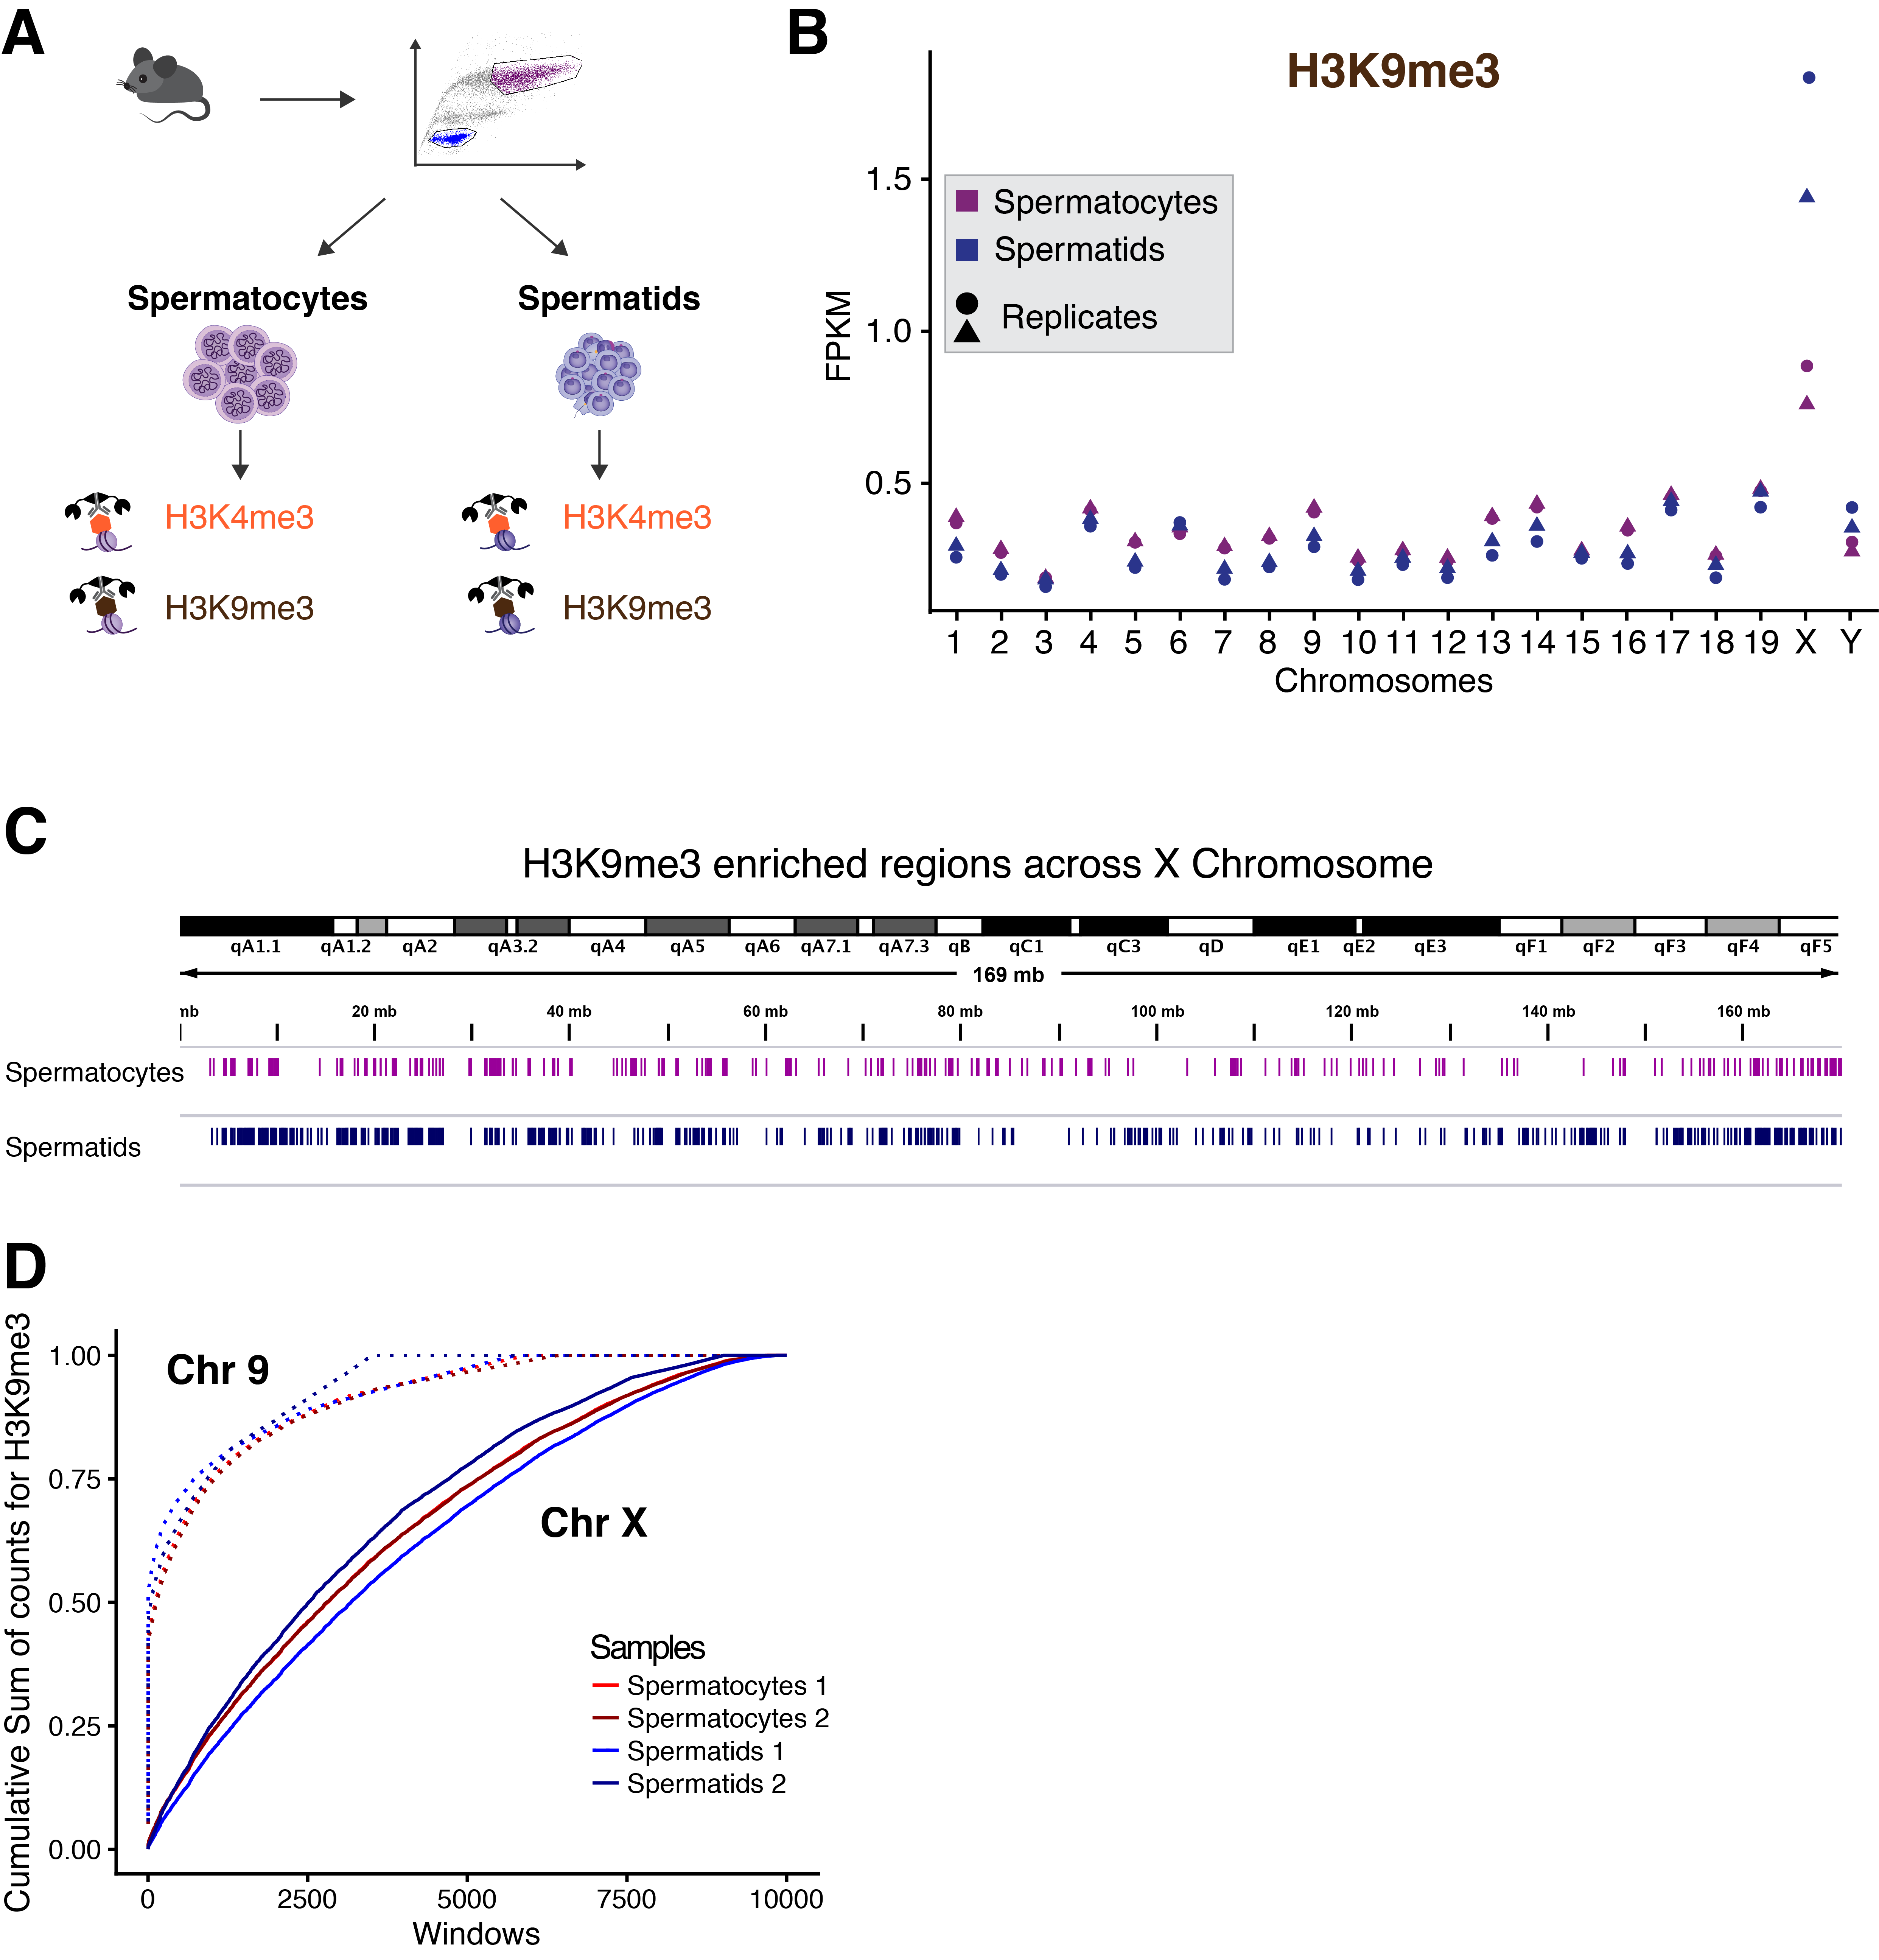
\includegraphics[width=\textwidth]{Fig_12.png}
\caption[\Gls{scDNA-Seq} allows detection of SNVs and CNVs between individual cells]{\textbf{\Gls{scDNA-Seq} allows detection of SNVs and CNVs between individual cells.}\\
Individual nuclei are captured in 96-well plates and directly lysed or fixated for multiplexing. Whole genome amplification (WGA) can be performed using MDA, MALBAC or SCOMP resulting in amplified genome segments. Depending on the biological question, whole genomes are either sequenced thoroughly to detect single nucleotide variants (SNVs) while shallow sequencing can be used to detect copy number variations (CNVs).}
\label{fig0:scDNA-Seq}
\end{figure}

\vspace{-5mm}

\subsubsection{Single-cell RNA sequencing}

Initial approaches to quantify mRNA abundance within single cells included targeted microfluidic-based single-cell RT-PCR \citep{Warren2006} and whole-transcriptome read-outs of hand-picked cells \citep{Tang2009}. Methods of cell capture range from micromanipulation \citep{Grindberg2014} and laser capture microdissections \citep{Frumkin2008} as targeted methods with low throughput to  \gls{FACS} \citep{Hayashi2010, Dalerba2011, Jaitin2014}, microfluidics \citep{Trapnell2014, Treutlein2014} and microdroplets \citep{Klein2015, Macosko2015} as high-throughput approaches \textbf{(Fig.~\ref{fig0:scRNA-Seq})}. More broadly, \gls{scRNA-Seq} approaches can be grouped into valve-, droplet- or well-based strategies \citep{Prakadan2017}. \\

A variety of scRNA-Seq protocols have been published that utilize different methods for mRNA reverse transcription, cDNA amplification and library preparation. All of these commonly used techniques for scRNA-Seq select and reverse transcribe mRNA (poly(A) tailing). The initial protocol introduced by Tang \textit{et al}, 2009 \citep{Tang2009} was improved by incorporating a template switching mechanism at the 5' end of the mRNA thus reducing the 3' sequencing bias present in previous methods \citep{Islam2011} (see below and \textbf{Fig.~\ref{fig0:scRNA-Seq}}). This \gls{STRT} method shows 5' bias in read mapping was later modified for full-length transcript detection (SmartSeq \citep{Ramskold2012} and SmartSeq2 \citep{Picelli2013}). CEL-Seq \citep{Hashimshony2012} and CEL-Seq2 \citep{Hashimshony2016} uses in vitro transcription (IVT) to linearly amplify cDNA prior to sequencing as opposed to exponential amplification in other techniques. Protocols for sequencing library preparation have been optimized for Illumina, SOLiD or PacBio sequencing \citep{Kolodziejczyk2015review}. \\

During scRNA-Seq minute amounts of mRNA are captured and amplified generating a high degree of technical noise, which distorts quantification of true biological variability. To account for this, a set of external RNAs developed by the \gls{ERCC} \citep{Rna2005} can be added to the cell lysate. Based on the reads mapped to ERCC spike-ins, technical noise can be removed from total expression variability \citep{Brennecke2013, Vallejos2015BASiCS}. Another way to reduce noise derived from amplification biases in scRNA-Seq experiments is to tag each mRNA molecule with a \gls{UMI} \citep{Kivioja2011, Islam2014}.\\

One example for a commercially available platform to capture individual cells and perform lysis, reverse transcription and pre-amplification of cDNA is the Fluidigm\textsuperscript{\textregistered{}} C1 system. Individual cells are loaded into \glspl{IFC}, also termed "chips", that allows capturing 96 to 800 cells. Depending on the size of the cells, this system offers chips with different capture well sizes. Each well can be microscopically inspected to differentiate between empty capture sites and single cells \citep{Kolodziejczyk2015review}. The C1 system uses the SMARTer\textsuperscript{\textregistered{}} chemistry to capture poly(A) mRNA with modified oligo(dT) primer. Next, the \gls{RT} reverse transcribes from the 3' to the 5' end of the mRNA and adds non-templated deoxycytidines to the 3' end of the cDNA. The template-switch primer contains guanosines at its 3' end that base-pair with the deoxycytidines on the cDNA to create an extended template. The RTase extends to the end of the template-switch primer. This produces single-stranded cDNA that contains the SMARTer tag sequence, the 3' end of the mRNA, the full-length transcript up to the 5' end of the mRNA, and the reverse complement of the SMARTer tag sequence. Amplification of this cDNA is performed by PCR on the chip \cite{Fluidigm2015}. After pre-amplification, the cDNA is collected and prepared for sequencing.\\

In parallel to extending scRNA-Seq protocols to robustly capture mRNA transcripts, efforts have been made to increase the throughput of this technology. Jaitin \emph{et al.}, 2014 introduced \gls{MARS-Seq} to sequence over 4000 cells of the mouse spleen. MARS-Seq captures cells in 384 well plates and labels transcripts of each cell with a combination of 2 random barcodes. This multiplexing strategy is performed using a liquid handling robot and cells can be pooled for sequencing library preparation which reduces costs and time effort \citep{Jaitin2014}. The first large-scale technique that captures tens of thousands of cells has been introduced by Fan \emph{et al.} in 2015. Here, 10,000 cells are captured in a 100,000 microwell surface. Additionally, barcoded beads are loaded into the surface until saturation. This Cyto-Seq approach is similar to the later on introduced Seq-Well technology \citep{Gierahn2017}. Each bead is coated with barcodes containing a unique sequence, a bead-specific barcode, a UMI and a oligo(dT) primer. After cell lysis and mRNA capture, beads are pooled and cDNA synthesis can be performed prior to sequencing \citep{Fan2015}. In the same year, the inDrop and Drop-Seq technologies were introduced \citep{Klein2015, Macosko2015}. Both technologies use microfluidic platforms to merge droplets containing barcodes, lysis and reverse transcription reagents with droplets containing cells. Similar to the above described Cyto-Seq \citep{Fan2015}, after lysis and mRNA capture, droplets are pooled for sequencing. The main difference is that cell-specific barcodes in Drop-Seq are bound to beads and to a polyacrylamide mesh in inDrop.  \\ 

\begin{figure}[!h]
\centering
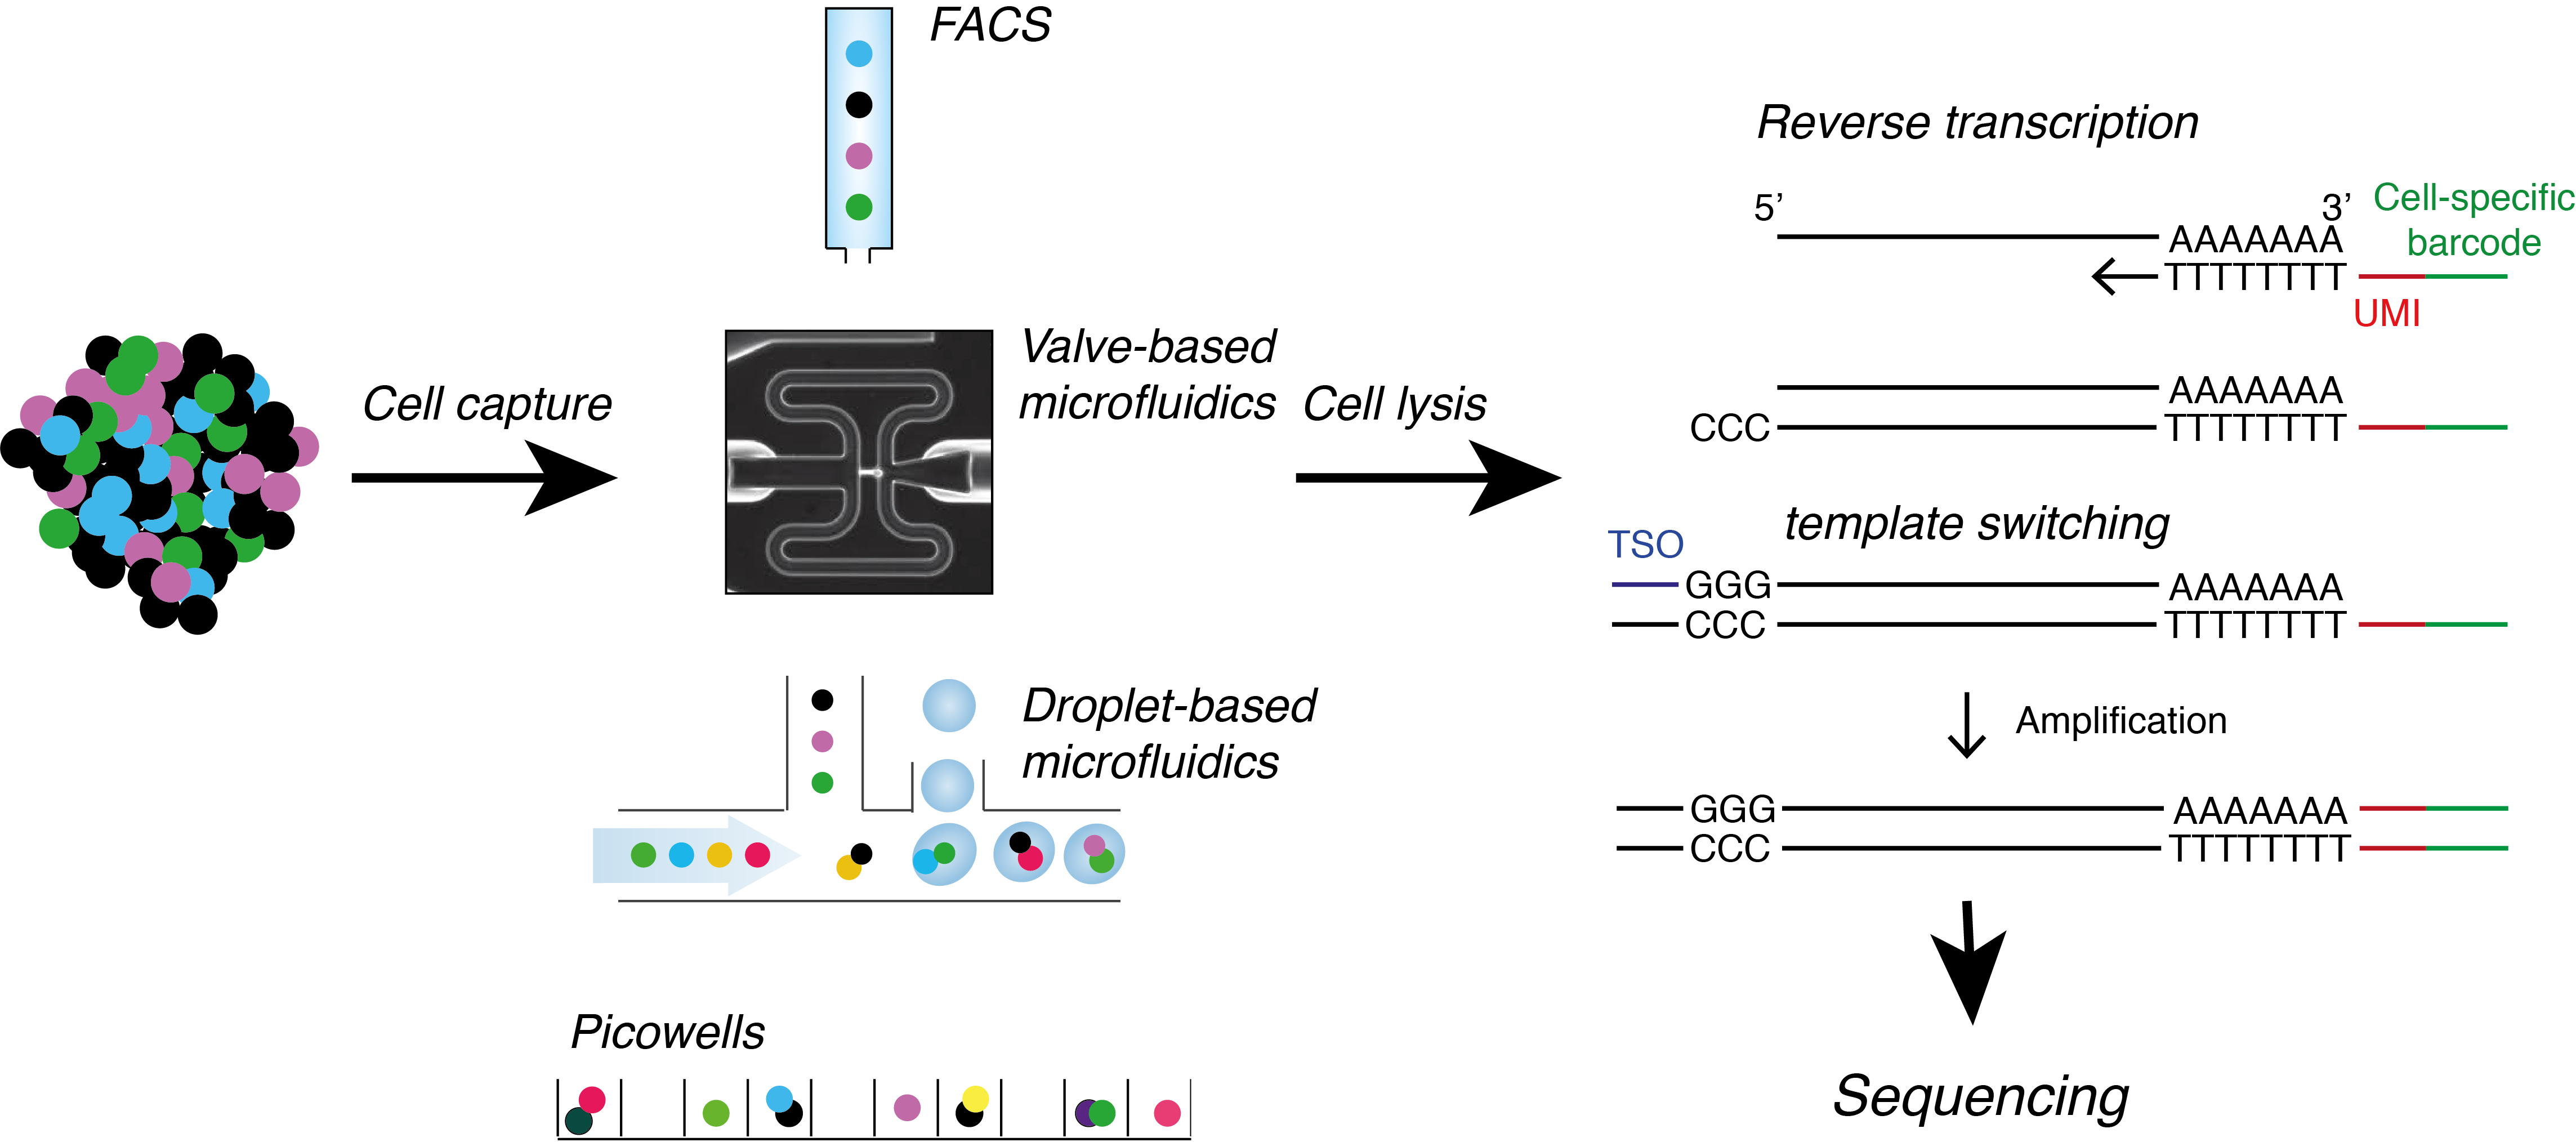
\includegraphics[width=\textwidth]{Fig_13.png}
\caption[Workflow for scRNA-Seq technologies]{\textbf{Workflow for scRNA-Seq technologies.}\\
Single cell suspensions are obtained by tissues dissection and dissociation. Commonly used cell capture technologies include fluorescence-activated cell sorting (FACS), valve-based microfluidics (Fluidigm\textsuperscript{\textregistered{}} C1 system), droplet-based microfluidics (10X Genomics\textsuperscript{\textregistered{}} system), or picowells. After cell capture and lysis, poly(dT) oligos capture mRNA prior to reverse transcription. In the case of droplet-based cell capture, ploy(dT) oligos are tagged with a unique molecular identifier (UMI) and a cell-specific barcode. \Gls{RT} generates cDNA from the template RNA. One strategy for RT is the template-switching protocol where the reverse transcriptase adds three cytidines at the 5' end of the template. A \gls{TSO} binds to the cytidines and allows amplification from the 5' end. After cDNA amplification, libraries are prepared for sequencing. For this, transposase degrades full length transcripts and Illumina sequencing primers are added (C1 system). In the case of the 10X Genomics system, the first read has been added next to the cell-specific barcode while the second read is added after cDNA fragmentation. This protocol shows a 3' bias.}
\label{fig0:scRNA-Seq}
\end{figure}

\newpage

10X Genomics\texttrademark{} has introduced a platform that uses these concepts to generate hundreds of thousands of Gel beads in EMulsions (GEM). Around 80\% of generated oil droplets capture barcoded gel beads in 8 channels in parallel. Each barcode consists of a sequencing adapter and primer, a 14bp sequence from a pool of 750,000 barcodes, a 10bp UMI and a 30bp poly(dT) oligotide to capture poly(A) mRNA \citep{Zheng2017}. GEMs are fused with individual cells at a low concentration and cell lysis begins instantaneous. mRNA molecules are capture by the poly(dT) barcode and enzymes needed for \gls{RT} are released from the gel beads. After RT, each cDNA contains a transcript specific UMI and a GEM specific barcode making demultiplexing possible \textbf{(Fig.~\ref{fig0:scRNA-Seq})}. Barcoded cDNA is pooled for PCR amplification and library preparation \citep{Zheng2017}.\\

Methods that even further increased the throughput of scRNA-Seq include \gls{SPLiT-Seq} and sci-RNA-Seq. Similar to sci-DNA-Seq (see above) these technologies are based on combinatorial indexing of mRNA in fixed cells or nuclei. Sci-RNA-Seq tags transcripts during two rounds of indexing with UMIs and a combination of two cell specific barcodes \citep{Cao2017}.  SPLiT-Seq on the other hand performs transcript tagging during 4 cycles adding 4 barcodes \citep{Rosenberg2018}. In that way, around 1 million cells can be uniquely labelled. At this stage the limiting factor is sequencing to obtain high-resolution whole transcriptomes of each cell.	These approaches as well as the recently developed \gls{DroNc-Seq} also allow sequencing mRNA from nuclei which is the preferred method for clinical samples, archived materials, and tissues that cannot be readily dissociated \citep{Habib2017}. 


\subsubsection{Single-cell epigenomics}

Single-cell epigenomic methods capture the chromatin state, histone modifications and DNA methylation state of individual cells and allow quantification of epigenetic variability across a population of cells \textbf{(Fig.~\ref{fig0:scEpigenomics})} \citep{Clark2016}. To observe methylation states of CpG motifs, \gls{scBS-Seq} involves the extraction of genomic DNA and cytosine to uracil bisulfite conversion prior to library preparation. 5-methylcytosine remains intact during conversion \citep{Smallwood2014, Farlik2015}. The throughput of this approach was scaled up by combinatorial indexing of fixed nuclei (i) prior to bisulfite conversion similar to sci-DNA-Seq and (ii) during PCR amplification (sci-MET-Seq) \citep{Basque2017}. \Gls{scRRBS-Seq} first enzymatically digests genomic DNA prior to bisulfite conversion. CpG-rich fragments can be enriched and amplified via ligated adapters before high-throughput sequencing \citep{Guo2013}. Extending the read-out of scBS-Seq and scRRBS-Seq, \gls{sc5hmC-Seq} captures the first oxidative product of CpG sites towards de-methylation and therefore cellular variation of methylation dynamics. Instead of bisulfite conversion, 5hmC sites are glucosylated before enzymatic digestion and adapter ligation \citep{Mooijman2016}. \\

To measure histone modifications or transcription factor binding dynamics on the single-cell level, digested chromatin from individual cells is tagged with barcodes prior to \gls{IP} during \gls{scChIP-Seq} \textbf{(Fig.~\ref{fig0:scEpigenomics})}. With this droplet-based method, variable chromatin signatures were detected across a population of embryonic stem cells based on the \gls{H3K4me2} mark \citep{Rotem2015}. 

\begin{figure}[!h]
\centering
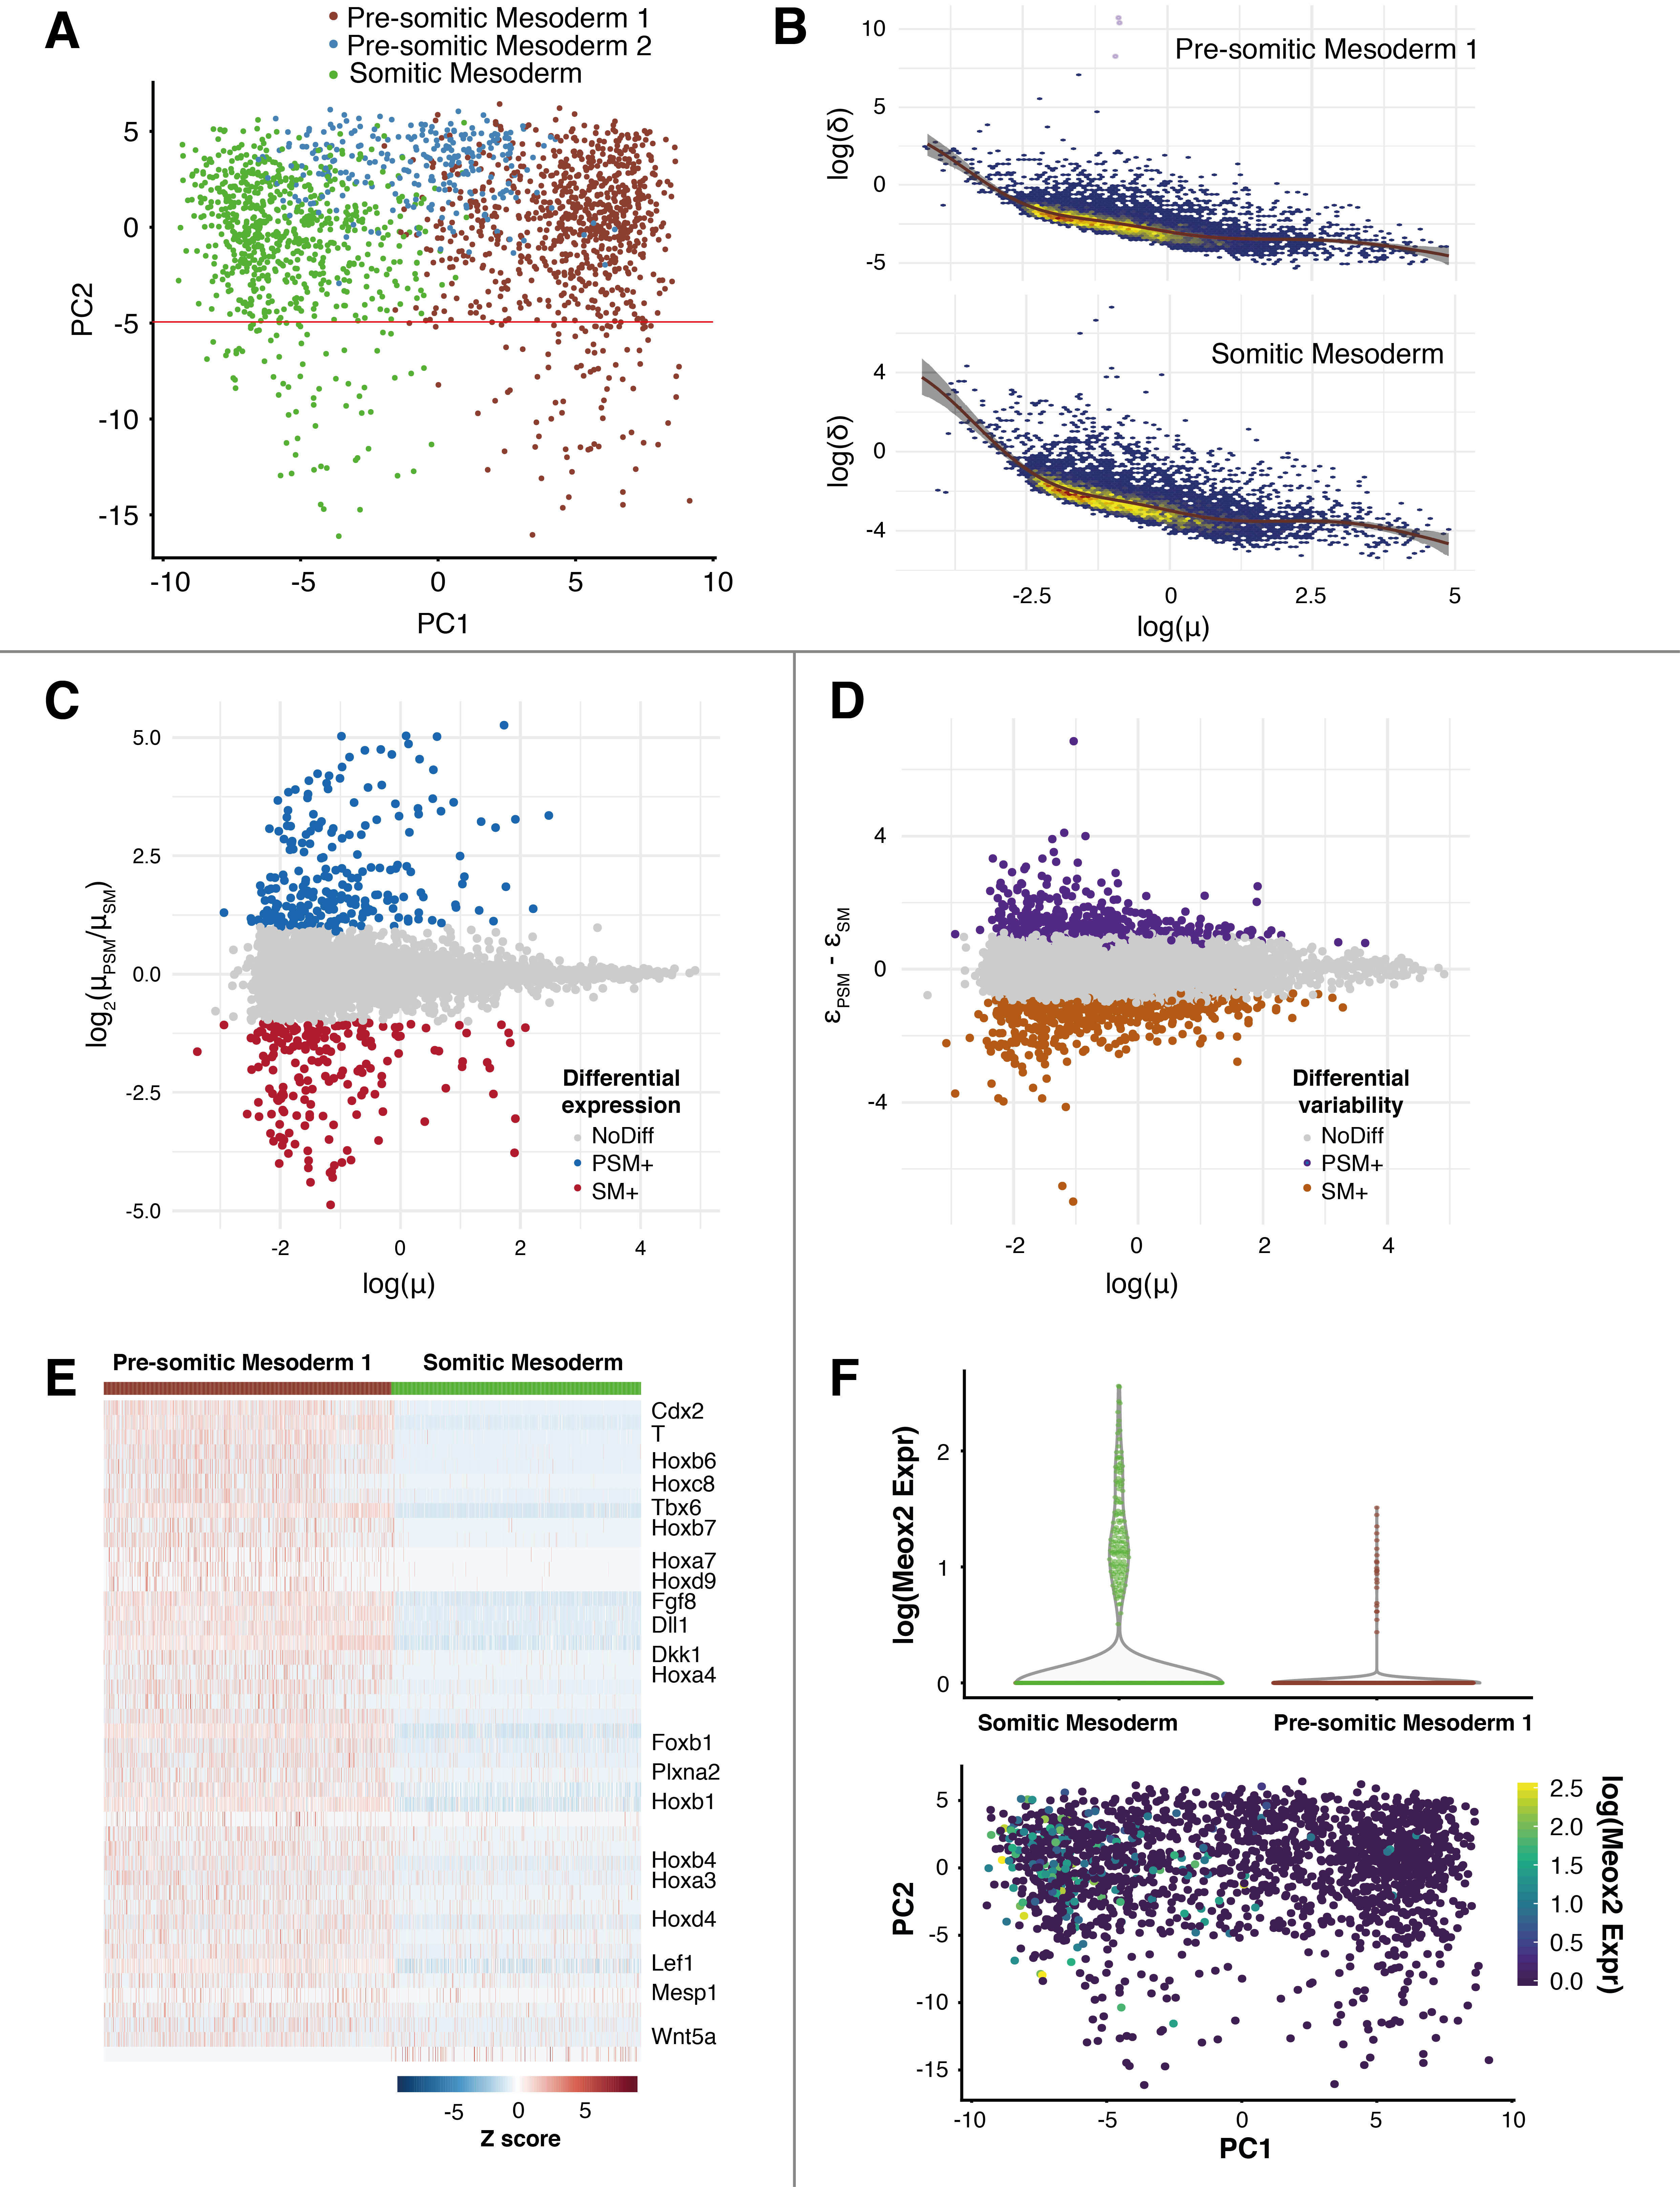
\includegraphics[width=\textwidth]{Fig_14.png}
\caption[Single-cell epigenomics to study chromatin structure and modifications]{\textbf{Single-cell epigenomics to study chromatin structure and modifications.}\\
Single-cell epigenomic technologies are used to study variation in DNA methylation, histone modifications, chromatin structure and nucleosome positioning across individual cells.}
\label{fig0:scEpigenomics}
\end{figure}

Other epigenomic approaches focus on estimating the patterns of open chromatin by capturing chromatin accessibility \textbf{(Fig.~\ref{fig0:scEpigenomics})}. \Gls{scATAC-Seq} captures individual cells on \glspl{IFC} before inserting sequencing adapters into accessible regions via the prokaryotic Tn5 transposase and pre-amplifiation. After library collection, cell-specific barcodes are added via a second round of PCR prior to sequencing \citep{Buenrostro2015}.  Capturing cells in IFCs before barcoding limits the throughput to around tens or hundreds of cells at one time. Combinatorial indexing by tagging cells with barcodes in a two step process increases throughput for scATAC-Seq to thousands of cells \citep{Cusanovich2015}. An alternative approach to measure open chromatin involves the digestion of DNA with DNase I (Pico-Seq). The resulting small fragments undergo end-repair, adaptor ligation and PCR amplification in the presence of circular carrier DNA to avoid the loss of minute amount of fragments \citep{Jin2015}. Similarly, nucleosome positioning can be detected by using the GpC-specific DNA \gls{MTase} M.CviPI to methylate cytosines of GpC motifs in regions where DNA is accessible. Individual cells are isolated and their DNA digested prior to bisulfite conversion. Patterns of methylated and unmethylated GpCs indicate the positioning of nucleosomes along the DNA \citep{Small2014}.\\

Single-cell technologies to study large-scale chromosome structure include \gls{DamID} \citep{Kind2015}, a method to identify lamina-associated domains, and single-cell \gls{HiC} \textbf{(Fig.~\ref{fig0:scEpigenomics})} \citep{Nagano2013}. Similar to sci-DNA-Seq, sci-RNA-Seq, sci-ATAC-Seq and sci-MET-Seq, sci-Hi-C uses multiplexing of fixated nuclei after digestion to insert (i) a biotinylated bridge adapter and later on a second adapter after lysis \citep{Ramani2017}. This technology allows the demultiplexing of thousands of cells after bulk-HiC-like processing. 

\subsubsection{Multi-omics approaches}

In recent years, some of the above described techniques were combined to measure transcriptomic, genomic, epigenomic and proteomic (“multi-omic”) features of single cells in parallel \citep{Macaulay2017}. The first approach for combinatorial \gls{DR-Seq} from the same cell amplifies genomic DNA and cDNA derived from reverse transcribed mRNA in one reaction step to avoid losses. After initial amplification, the sample is split to further process gDNA and cDNA separately. PCR amplification increases the amount of gDNA while IVT amplifies cDNA prior to sequencing \citep{Dey2015}. An alternative approach, \gls{GT-Seq}, firstly separates gDNA and mRNA before whole-transcriptome and whole-genome amplification. Biotinylated oligo(dT) primers capture mRNA and are coupled to streptavidin coated beads. Once mRNA and gDNA is separated, the SmartSeq2 protocol performs whole-transcriptome amplification while MDA or PicoPlex approaches can be used to amplify gDNA prior to sequencing \textbf{(Fig.~\ref{fig0:multiomics})} \citep{Macaulay2015}.\\

\begin{figure}[!h]
\centering
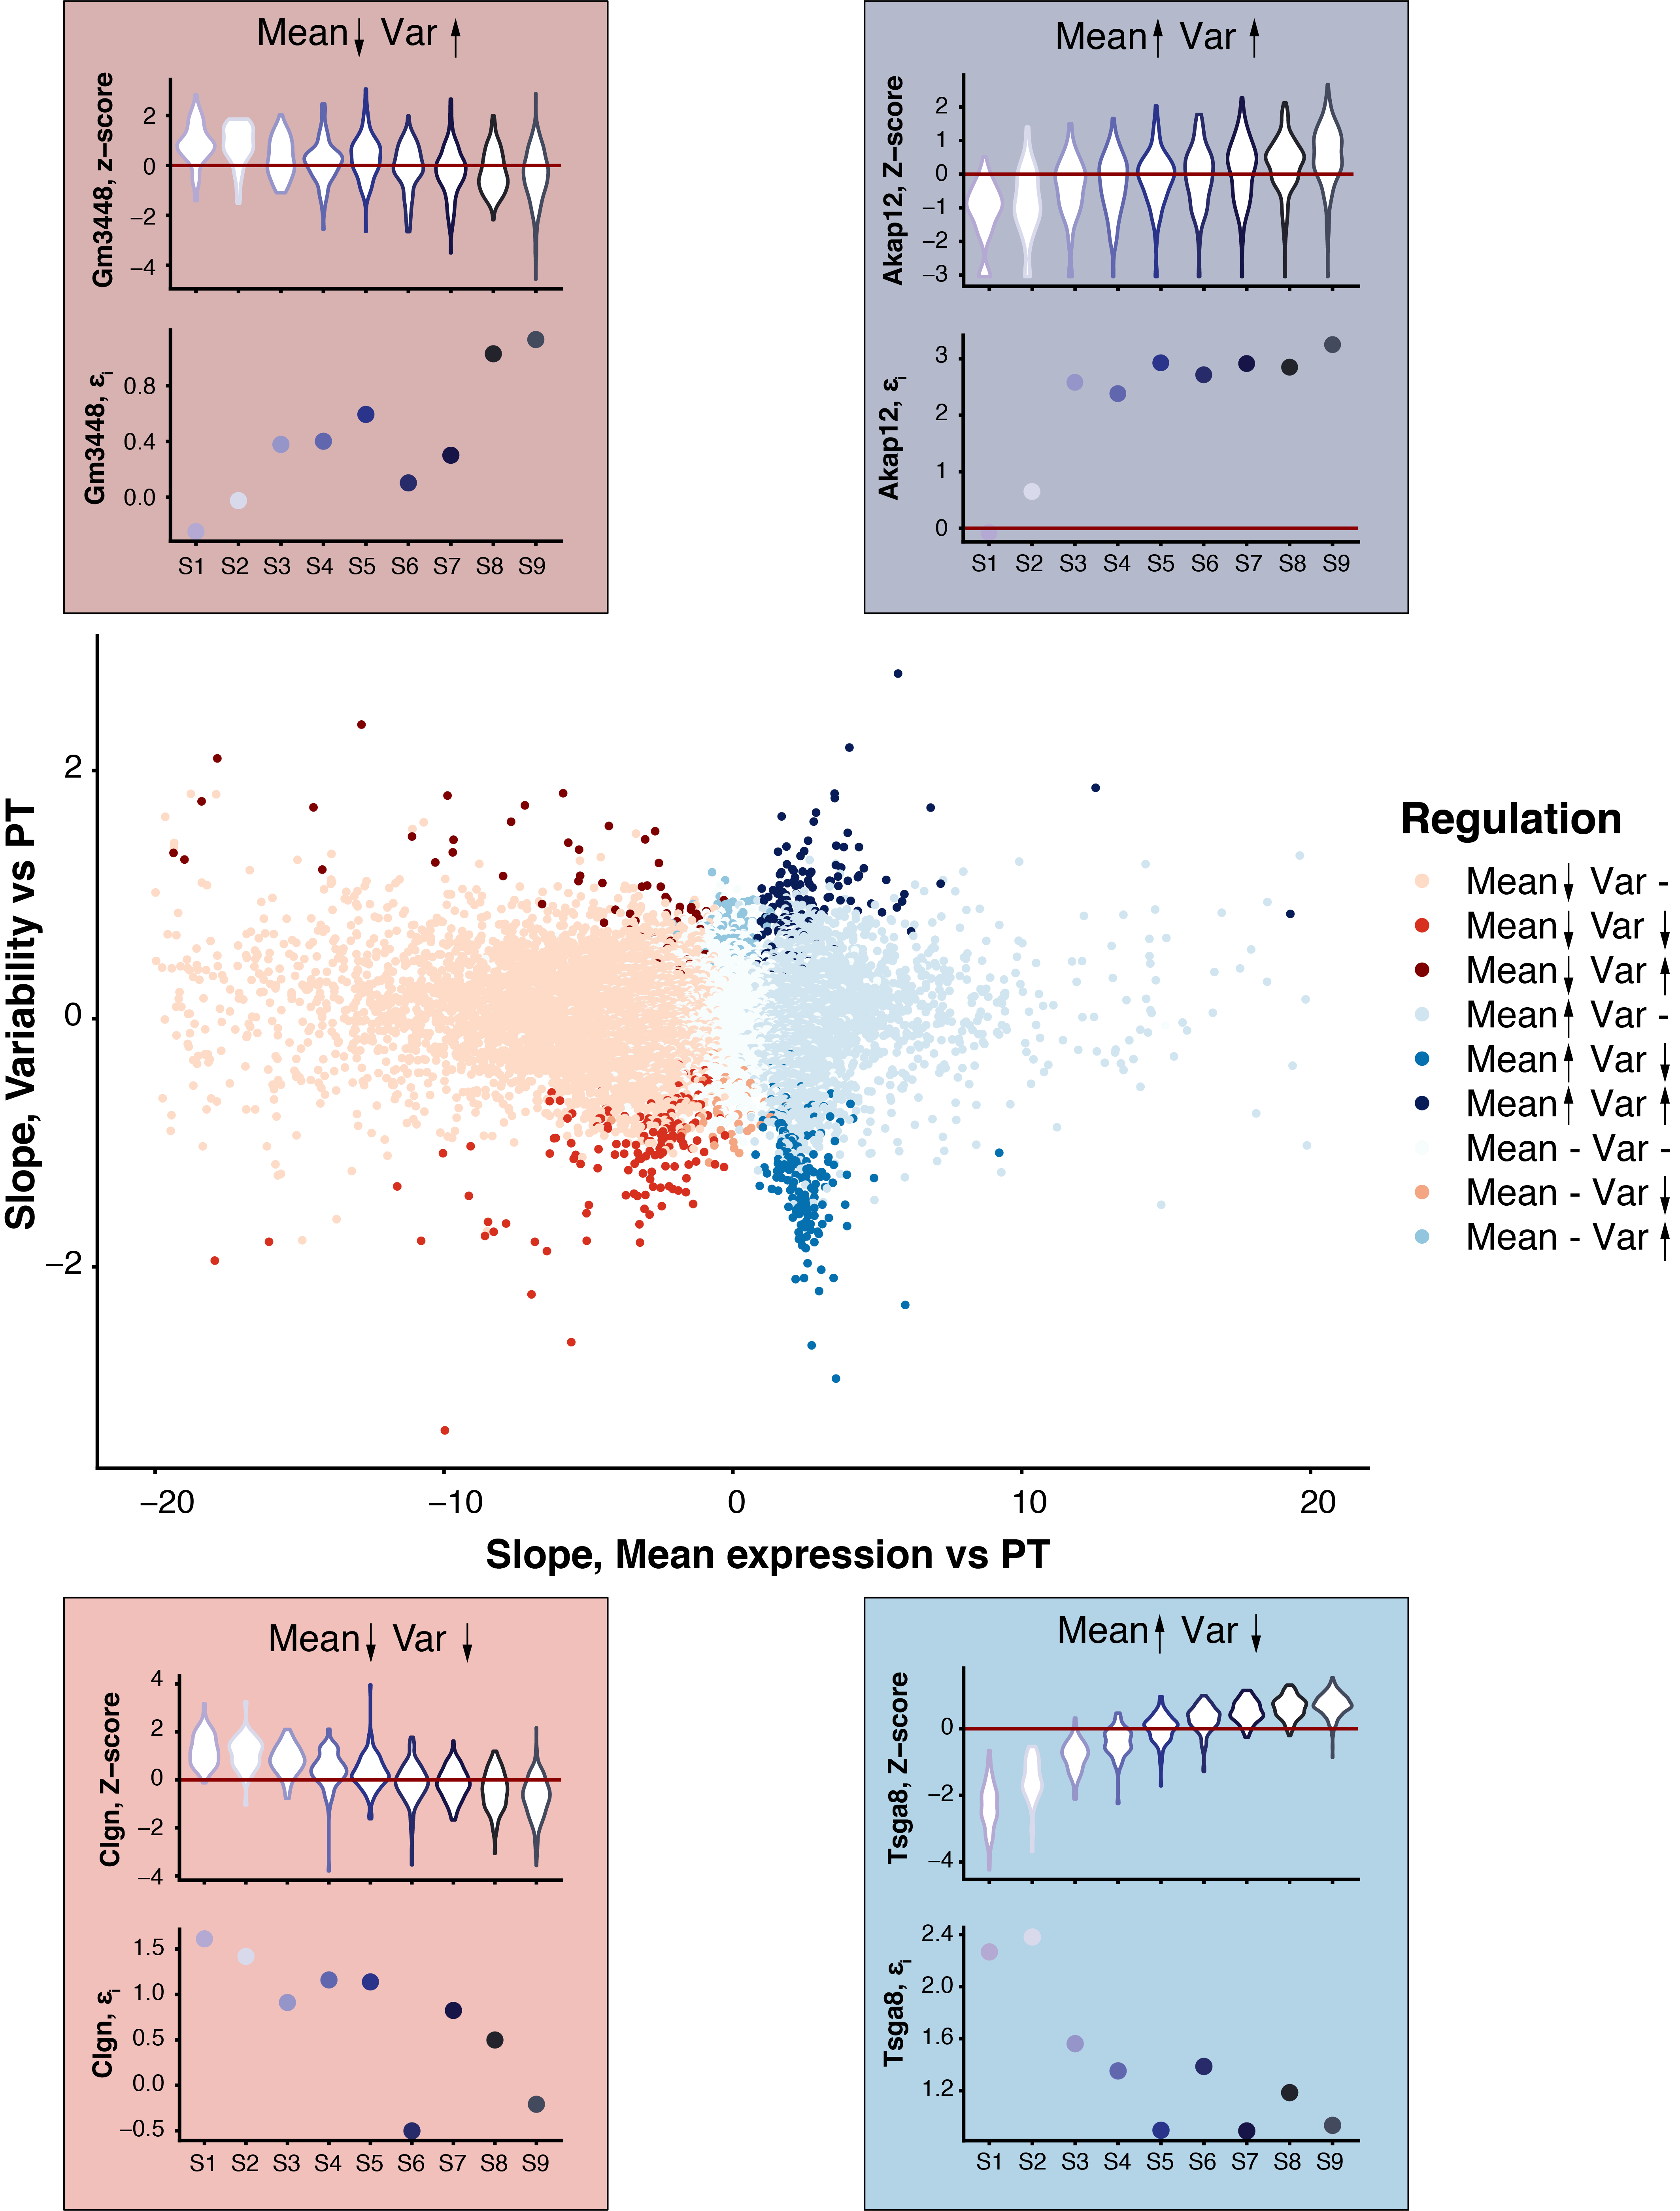
\includegraphics[width=\textwidth]{Fig_15.png}
\caption[Single-cell multi-omic approaches]{\textbf{Single-cell multi-omic approaches.}\\
Single-cell DNA and RNA-Seq either directly separates RNA and DNA or pre-amplifies both prior to separation. Measuring RNA and protein abundance from individual cells is done after physical separation followed by either oiligonucleotide tagging of proteins or isotope tagging of RNA molecules. For methylome and transcriptome sequencing, DNA and RNA are separated prior to RNA sequencing and bisulfite conversion.}
\label{fig0:multiomics}
\end{figure}

Similarly, \gls{scMT-Seq} initially separates genomic DNA from mRNA. The scBS-Seq protocol is applied to isolated gDNA and identify methylated CpG positions while mRNA was amplified via the SmartSeq2 protocol \citep{Angermueller2016a}. The scM\&{}T-Seq method has been extended to detect accessible chromatin regions in parallel to capturing methylated CpG sites and whole-transcriptome information. Prior to bisulfite conversion of gDNA, GpC sites are methylated by MTase in nucleosome spares regions \textbf{(Fig.~\ref{fig0:multiomics})} \citep{Pott2017, Clark2018}.\\
 
Attempts have been made to capture $\sim$96 mRNAs in combination with proteins within individual cells. After cell lysis, samples are split to process mRNA and protein separately. mRNA is reverse transcribed and pre-amplified prior to \gls{qPCR} while oligonucleotide tagged antibodies bind to proteins. The free 3’-ends are complementary and can be extended by polymerization to create a DNA reporter molecule. Similar to mRNAs, these molecules are detected using qPCR \citep{Darmanis2016}. This method has been scaled up by integration of droplet digital PCR \citep{Albayrak2016}. Alternatively, proximity ligation assay for RNA allows isotope tagging of RNA molecules, which are detected in parallel to proteins via mass cytometry \textbf{(Fig.~\ref{fig0:multiomics})} \citep{Frei2016}.

\subsection{Imaging approaches}

Similar to single-cell sequencing, RNA or protein imaging approaches quantify noise in biological systems \citep{Harton2017a}. Initial studies that addressed the extend of biological noise in bacterial populations used the expression of fluorescent proteins under controlled by promoters of interest (reporter assays) to quantify expression noise \citep{Elowitz2002, Blake2003}. Later on, \gls{smFISH} was developed to capture variation in mRNA abundance across multiple cells \citep{Fang2013a, Lyubimova2013, Sanchez2013} and in whole organs \citep{Yang2014b}. Furthermore, the combination of fluorescently labeled proteins and smFISH allow the detection of co-variation between protein and mRNA levels within individual cells \citep{Taniguchi2011}. High-throughput automated smFISH of target RNAs in thousands of wells \citep{Battich2013} identified nuclear retention of RNAs as control mechanism to reduce cytoplasmic transcript variability \citep{Battich2015a}. Moreover, computerized image analysis and supervised machine learning extracts hundreds of cellular features from microscopy images and can therefore dissect variation of biological processes such as virus infection \citep{Snijder2009}.\\

\begin{figure}[!h]
\centering
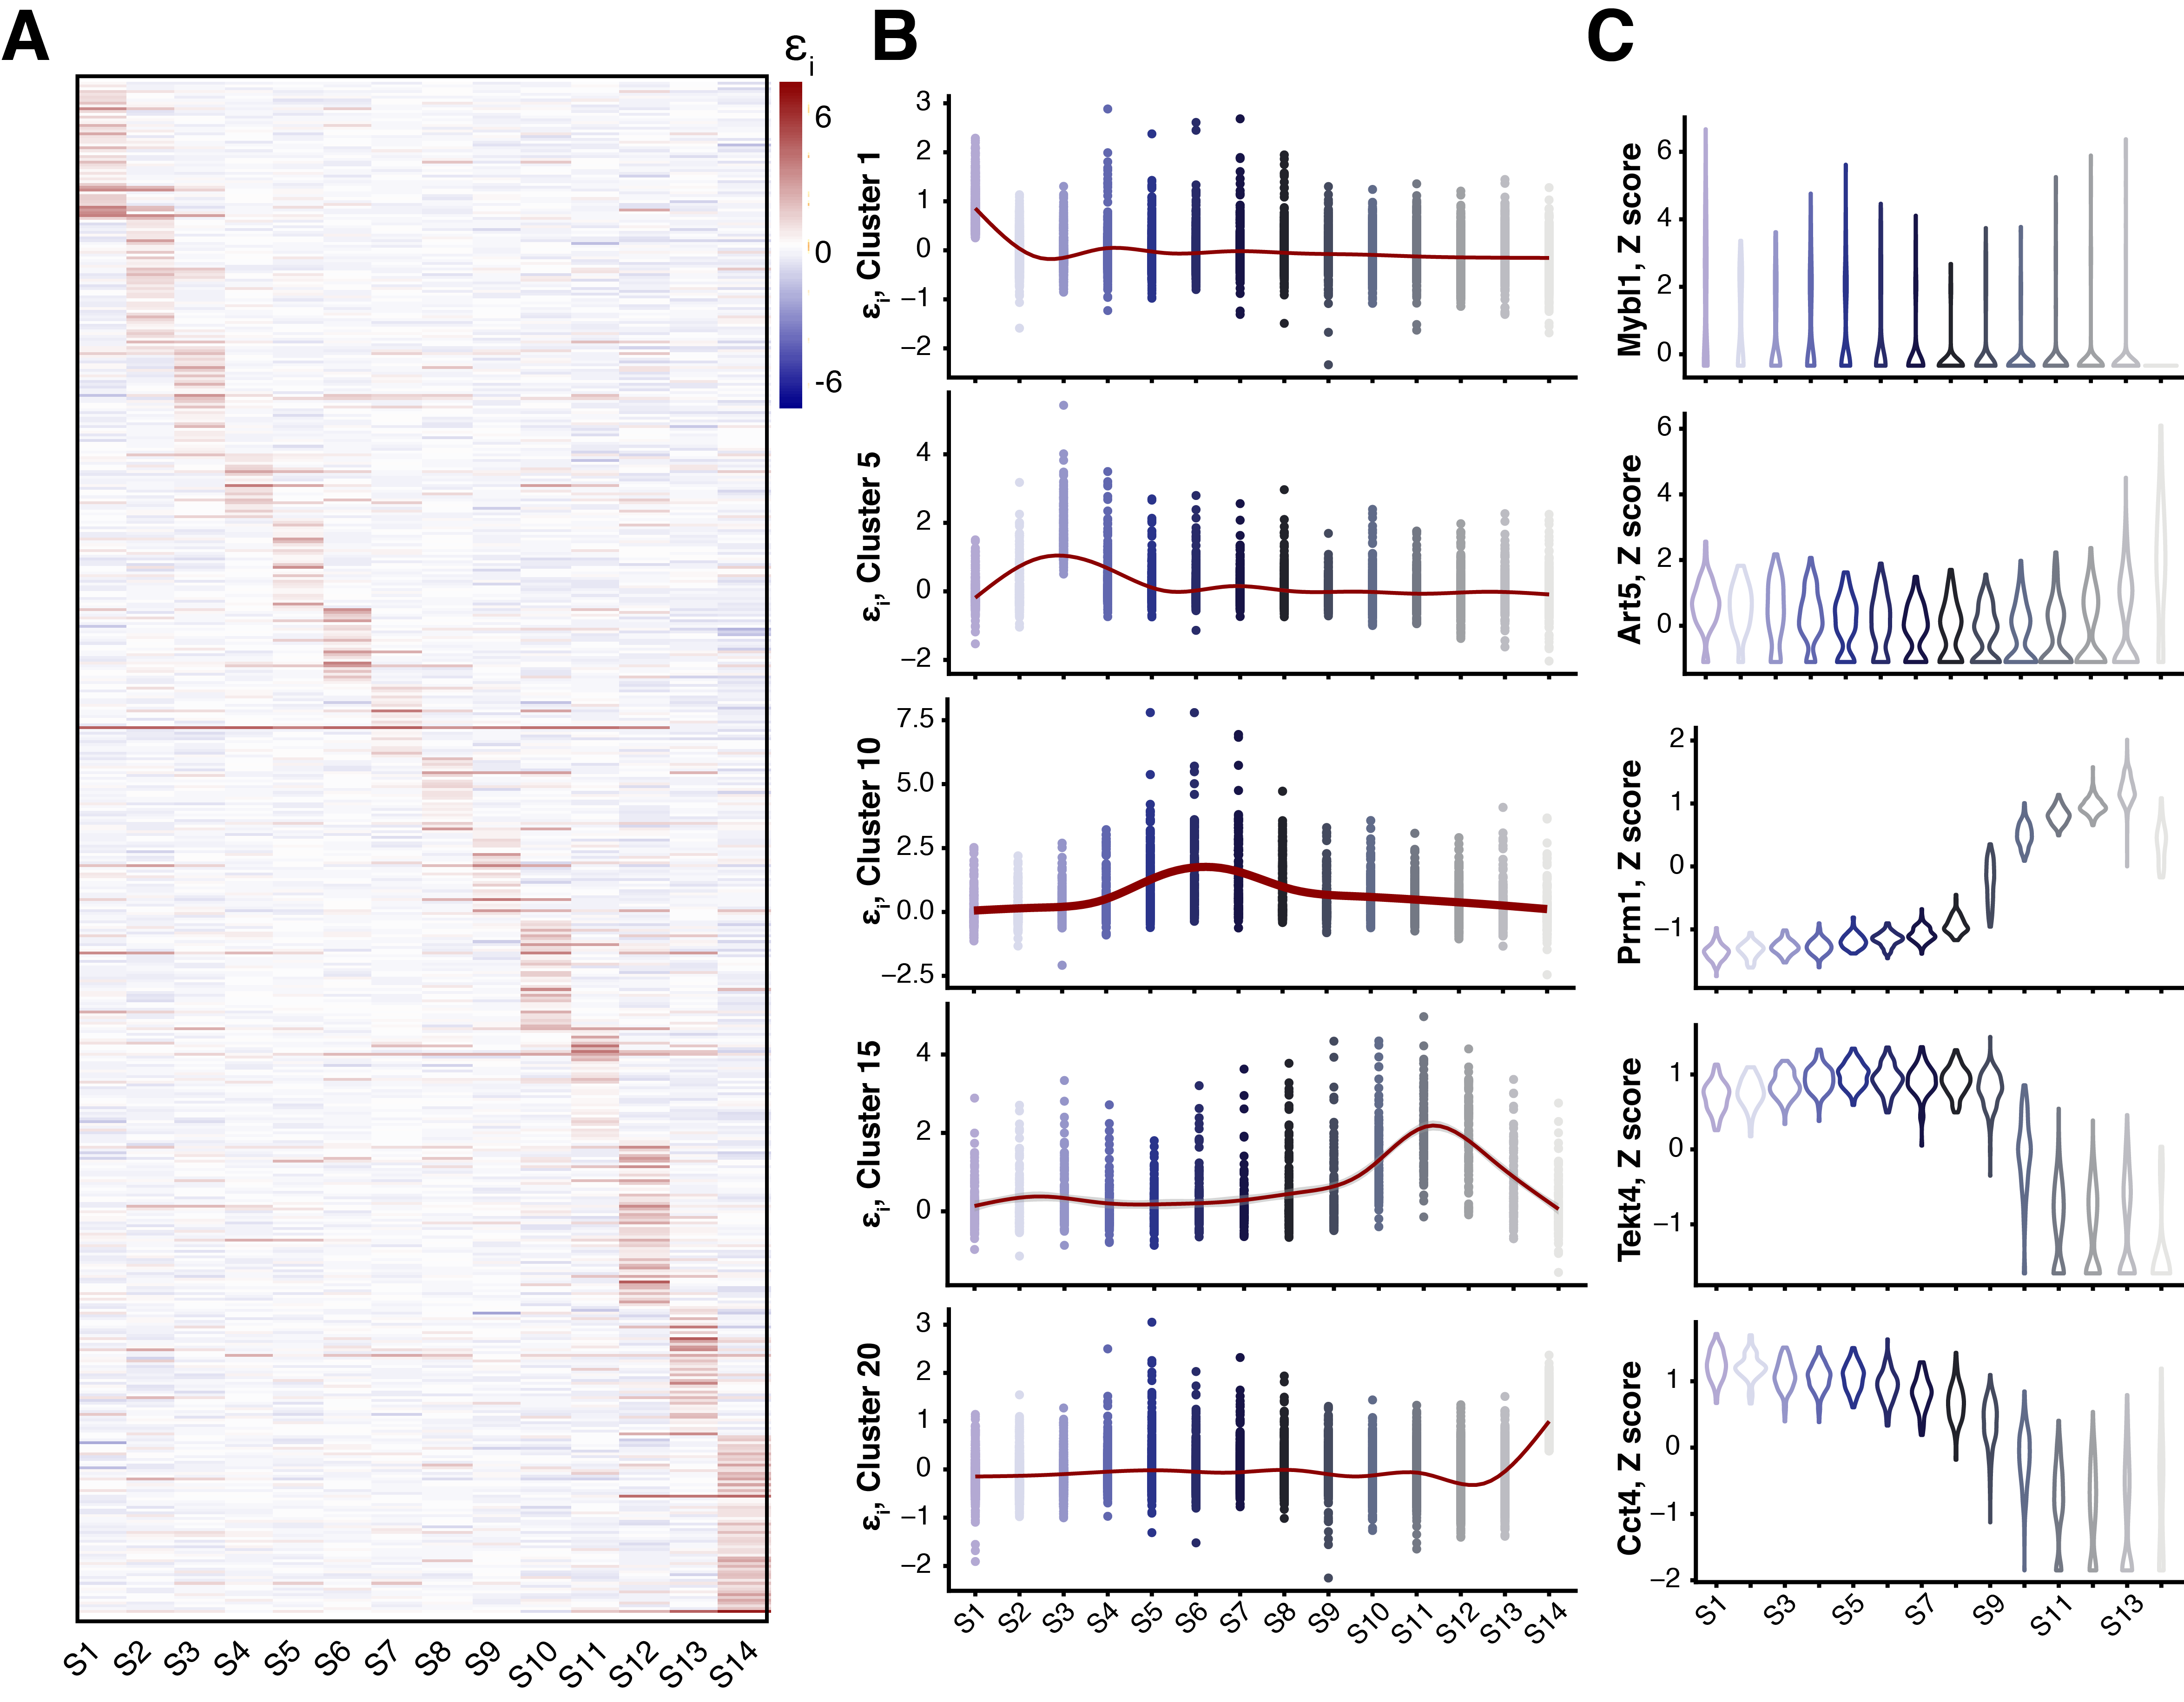
\includegraphics[width=\textwidth]{Fig_16.png}
\caption[MERFISH-type spatial transcriptomics]{\textbf{MERFISH-type spatial transcriptomicsd.}\\
Each transcript species is tagged with encoding probes that contain a sequence to recognise the RNA and multiple read-out sequences. During each hybridisation cycle, individual read-out probes hybridise with their specific sequences on the encoding probes. After multiple rounds of hybridisation and imaging, individual RNA transcripts can be decoded.}
\label{fig0:MERFISH}
\end{figure}

\newpage

The development of super-resolution microscopy allows detection of fluorophores that are spaced less than 100nm apart \citep{Sydor2015}. By combining \gls{STORM} and combinatorial labeling of RNA inside the cell, multiple transcripts from different genes can be visualized \citep{Lubeck2012}. This approach has been advanced to measure hundreds to thousands of RNA species per cell. \Gls{MERFISH} hybridizes encoding probes to target RNAs prior to $N$ rounds of combinatorial labelling using fluorescently labelled read-out probes \textbf{(Fig.~\ref{fig0:MERFISH})}. MERFISH uses an encoding scheme that corrects for individual read-out errors based on a certain hamming distance between possible N-bit codes. Therefore, with 16 rounds of combinatorial labeling and a hamming distance of 4, 140 RNA species can be detected \citep{Chen2015}. A similar approach has been developed to profile spatial expression patterns in the mouse hippocampus (seqFISH) \citep{Shah2016}. By replacing the photobleaching step between consecutive rounds of combinatorial labelling with chemical cleavage and using multi-color imaging, the throughput of MERFISH can be increased \citep{Moffitt2016a}. Background fluorescence in tissue sections can be reduced by matrix-embedding of labelled RNA and cellular digestion \citep{Moffitt2016}.

\subsection{Computation modelling and quantification}

Previous research focused on the derivation of mathematical and computational frameworks to model transcriptional and translation dynamics in biological systems \citep{Tsimring2014}. In the simplest case, the central dogma of molecular biology defines that mRNAs are synthesized from DNA at rate $k_m$ and proteins are translated from mRNAs at rate $k_p$. Furthermore, mRNAs are degraded at rate $\gamma_m$ and proteins at rate $\gamma_p$. In a noise-free system, this dogma leads to the following \textbf{deterministic}, first-order differential equation describing the mRNA abundance ($m$) and protein abundance ($p$) over time:

\begin{equation}
\frac{dm}{dt}=k_m-\gamma{}_mm,\quad \frac{dp}{dt}=k_pm-\gamma{}_pp
\end{equation}

\doublespacing
\noindent Steady-state transcript counts in this simple, two-stage system are defined as $\langle{}m\rangle{}=\frac{k_m}{\gamma_m}$  and protein abundance as $\langle{}p\rangle{}=\frac{k_mk_p}{\gamma_m\gamma_p }$. The second moments for transcript and protein distributions are defined as: $\sigma^2=\langle{}m\rangle{}$ and $\sigma_p^2=\langle{}p\rangle{}\left[\frac{k_p}{\gamma_p+\gamma_m}+1\right]=\langle{}p\rangle{}\left[\frac{b}{1+\eta}+1\right]$, where $b=k_p/\gamma_m$  is the average number of proteins produced per transcript and $\eta=\gamma_p/\gamma_m$  \citep{Tsimring2014, Thattai2001}. mRNAs usually decay much faster than proteins. Therefore $\gamma_m\gg{}\gamma_p$ and $\sigma_p^2\cong\langle{}p\rangle{}\left[b+1\right]$ \citep{Thattai2001}.\\
For this system, the mean translational burst size can be described as the Fano factor $\frac{\sigma_p^2}{\langle{}p\rangle}\cong{}b+1\approx{}b$ and burst frequency is captured by the inverse squared coefficient of variation $\frac{\langle{}p\rangle{}^2}{\sigma_p^2}\approx{}\frac{\langle{}p\rangle{}}{b}=\frac{k_m}{\gamma_p}=a$. The latter assumes that mRNAs are directly translated as soon as they are produced \citep{Friedman2006}.\\

\onehalfspacing
\noindent To account for stochasticity in this system, probabilistic expressions of aforementioned equations have been described. The chemical master equation defines the time-evolution of the probability of observing a system containing $m$ mRNAs and $p$ proteins at time-point $t$:

\begin{align}
\frac{\partial{}P_{m,p}}{\partial{}t}&=k_n\left[P{m-1,p}-P_{m,p}\right]+\gamma_m\left[(m+1)P_{m+1,p}-mP_{m,p}\right] \nonumber \\
&+k_pm\left[P_{m,p-1}-P_{m,p}\right]+\gamma_p\left[(p+1)P_{m,p+1}-pP_{m,p}\right]
\end{align}

\noindent The stationary probability distribution for this discrete representation of the master equation has the form of a negative-binomial distribution:

\begin{equation}
P_p=\frac{\Gamma(a+n)}{\Gamma(n+1)\Gamma(a)}\left(\frac{b}{1+b}\right)^n\left(1-\frac{1-b}{1+b}\right)^a
\end{equation}

\noindent where $a$ represents the burst frequency, $b$ the mean burst size and $\Gamma(n)$ the Gamma function \citep{Shahrezaei2008}. Friedman \textit{et al.}, 2006 derived a stationary probability distribution from a continues form of the chemical master equation \citep{Friedman2006}. This solution takes the form of a Gamma distribution:

\begin{equation}
P_p=\frac{1}{b^a\Gamma(a)}n^{a-1} e^{-n/b}
\end{equation}

\noindent This simple system has also been extended to incorporate the ON-OFF switching of promoters \citep{Jones2014, Shahrezaei2008}. Extensive modeling and quantification of mRNA and protein abundance in prokaryotic and eukaryotic cell populations confirmed this negative binomial (over-dispersed Poissonian) relationship between protein variance and abundance \citep{Ozbudak2002, Bar-Even2006}. The over-dispersion in protein abundance arises from biological noise ($\eta_{tot}$), which can be decomposed into intrinsic ($\eta_{int}$) and extrinsic ($\eta_{ext}$) contributions ($\eta_{tot}=\eta_{int}+\eta_{ext}$) \citep{Swain2002, Fu2016}. These components can be directly computed when using a two reporter system controlled by identical promoters \citep{Elowitz2002}. \\

Classic mathematical approaches to model transcriptional and translational dynamics use simplified assumptions to be solved analytically. Similar to the described translational bursting, transcriptional bursting as observed in eukaryotic cells \citep{Raj2006} leads to an over-dispersion in mRNA transcripts. Furthermore, while most models focus on single promoter dynamics, cases in which multiple promoters and competitor sites dilute TF binding have only recently been addressed \citep{Das2015a}. The assumption that translation from mRNA follows a first-order process was extended by using a hyperbolic, Michaelis-Menten kinetic to model the translation process. This approach allows for continuous levels of ribosome occupancy on mRNAs \citep{VanDyken2017}. \\ 

While the models described above theoretically describe the expected distributions of proteins and mRNA across a population of cells, in practice, absolute measures (e.g. transcript counts or fluorescence intensity) have to be used to quantify variation across a population of cells. \\

\todo{Add Kims paper} \\

Previously, a variety of heterogeneity measures were computed to estimate biological noise. \\

In the simplest form, the variance $\sigma^2$, either calculated across all cells or across all expressing cells \citep{Shalek2014}, captures variability in RNA and protein abundance and scales linearly with mean expression $\mu$ \citep{Dey2015a}. The \gls{CV2} or the Fano factor are more widely used to measure heterogeneous RNA expression \citep{Brennecke2013, Jones2014} and protein abundance \citep{Newman2006}. Lowly expressed genes show higher levels of noise compared to highly expressed genes \citep{Brennecke2013}. Therefore, the CV$^2$ decreases with mean expression. To compare variability measures across different biological conditions where mean expression changes, regression approaches have been used to correct for the mean-variance relationship \citep{Kolodziejczyk2015cell, Fan2016}. \\
 
Other approaches directly model biological variability as the excess in dispersion after removing technical noise. Similar to the \citep{Brennecke2013} this over-dispersion measure decreases with increasing mean expression \citep{Vallejos2015BASiCS}. Moreover, heterogeneous expression can be captured by computing the Shannon entropy. Gene-specific entropy is defined as $H=-\sum_i{}p_i\log_2(p_i)$ where $p_i$ is the probability for a given gene being expressed in bin $i$. Binning across the expression counts can be done by choosing a fixed width \citep{Richard2016} or an adaptive width \citep{Stumpf2017}. Additionally, average pairwise distances between cells capture increasing or decreasing heterogeneity in cell populations \citep{Mohammed2017}. \\ 

In some cases, intrinsic variation in gene expression can be masked by large-scale extrinsic effects (e.g.~cell being in different cell-cycle stages). Methods have been developed to correct for these confounding effects to dissect otherwise hidden variation \citep{Buettner2015, Buettner2017}.
